\chapter{Návrh implementace}
Jak již bylo zmíněno na začátku práce, samotná implementace je rozdělena do dvou částí:
\begin{enumerate}
	\item Komunikace RaspberryPi přes rozšiřující desku UniPi s bezdrátovým modulem a pomocí něj s poskytnutými WM-Bus zařízeními.
	\item Zachytávání šifrované i nešifrované komunikace s WM-Bus zařízeními. Uložení, analýza a následná vizualizace zachycených dat. 
\end{enumerate}

Jelikož žádný z dostupných softwarů pro UniPi nepodporuje daný bezdrátový modul, ani UART zařízení obecně, je nutné tuto komunikaci implementovat již na úrovni operačního systému.

%%%%%%%%%%%%%%%%%%%%%%%%%%%%%%%%%%%%%%%%%%%%%%%%%%%%%%%%%%%
%%%%%%%%%%%%%%%%%%%%%%%%%%%%%%%%%%%%%%%%%%%%%%%%%%%%%%%%%%%
%%%%%%%%%%%%%%%%%%%%%%%%%%%%%%%%%%%%%%%%%%%%%%%%%%%%%%%%%%%
%%%%%%%%%%%%%%%%%%%%%%%%%%%%%%%%%%%%%%%%%%%%%%%%%%%%%%%%%%%

\section{Výběr OS}
Jako operační sytém je využita aktuální verze Raspbianu Jessie s datem vydání 2017-01-11. UART rozhraní se na RaspberryPi verze 1 a 2 nachází v \texttt{/dev/ttyAMA0}. To se ale v případě RaspberryPi 3 odkazuje na integrovaný BT modul a původní sériový port je zde v \texttt{/dev/ttyS0}. Samotné UART rozhraní je ale ve výchozím nastavení Raspbianu zakázáno.

Pro zpřístupnění UART rozhraní je nutné provést drobné úpravy jeho konfigurace:


\begin{enumerate}
	\item Nejdříve je nutné provést kompletní aktualizaci Raspbianu, tedy v konzoli spustit posloupnost příkazů:
	
	\begin{lstlisting}[style=MyCodeBash]
		sudo apt-get update
		sudo apt-get upgrade
		sudo apt-get dist-upgrade
		sudo apt-get rpi-upgrade	
	\end{lstlisting}
					
	\item Poté je potřeba v \texttt{/boot/config.txt} změnit položku \texttt{ENABLE\_UART} na hodnotu 1. Tím dojde k zpřístupnení sběrnice UART. Tato položka může být v budoucnu při aktualizaci Raspbianu přepsána, proto při prvním náznaku nefunkčnosti, je potřeba tuto položku zkontrolovat jako první.
	\item V souboru \texttt{/boot/cmdline.txt} je potřeba odebrat úsek textu \texttt{console=ttyAMA0, 115200}, aby při startování systému nedocházelo k výpisu do seríové linky. 
	\item V případě, že se jedná o RaspberryPi verze 3, je potřeba do \texttt{/boot/config.txt} dopsat položku \texttt{dtoverlay=pi3-miniuart-bt}, která zakáže BT na mini-UART a provede přemapování zpět na \texttt{/dev/ttyAMA0}. Tento krok je takto řešený z důvodu kompatibility, kdy je sériová komunikace směrována přes \texttt{/dev/ttyAMAO} nezávisle na použité verzi RaspberryPi.
\end{enumerate}

Po každém z těchto kroků je doporučován restart zařízení. Kroky byly otestovány pouze na výše zmíněné verzi Raspbianu a v jiných distribucích se monou mírně lišit. Úspěšnost provedení těchto kroků lze zkontrolovat pomocí zadání příkazu konzole 
	\begin{lstlisting}[style=MyCodeBash]
			sudo dmesg | grep tty
	\end{lstlisting}

jehož výstup by měl být následující:
					
	\begin{lstlisting}[style=MyCodeBash]
[    0.000974] console [tty1] enabled
[    0.130442] 20201000.uart: ttyAMA0 at MMIO 0x20201000 (irq = 81, base_baud = 0) is a PL011 rev2
	\end{lstlisting}
	\vspace{-20pt}


%%%%%%%%%%%%%%%%%%%%%%%%%%%%%%%%%%%%%%%%%%%%%%%%%%%%%%%%%%%
%%%%%%%%%%%%%%%%%%%%%%%%%%%%%%%%%%%%%%%%%%%%%%%%%%%%%%%%%%%
%%%%%%%%%%%%%%%%%%%%%%%%%%%%%%%%%%%%%%%%%%%%%%%%%%%%%%%%%%%
%%%%%%%%%%%%%%%%%%%%%%%%%%%%%%%%%%%%%%%%%%%%%%%%%%%%%%%%%%%

\section{Výběr programovacího jazyka}
Jelikož primárním jazykem využívaným na platformě RaspberryPi je Python, který již obsahuje knihovny pro sériovou komunikaci, je současný kód napsán v jazyce Python 3.

%%%%%%%%%%%%%%%%%%%%%%%%%%%%%%%%%%%%%%%%%%%%%%%%%%%%%%%%%%%
%%%%%%%%%%%%%%%%%%%%%%%%%%%%%%%%%%%%%%%%%%%%%%%%%%%%%%%%%%%
%%%%%%%%%%%%%%%%%%%%%%%%%%%%%%%%%%%%%%%%%%%%%%%%%%%%%%%%%%%
%%%%%%%%%%%%%%%%%%%%%%%%%%%%%%%%%%%%%%%%%%%%%%%%%%%%%%%%%%%

\section{Nastavení komunikačního modulu a čidla}

Před samotným vyčítáním dat bylo potřeba zjistit či nastavit přenosové parametry všech použitých zařízení:

\begin{itemize}
	\item Komunikační modul IQRF nastaven do módu T1 ve funkci skeneru.
	\item Čidlo Weptech je nastaveno do módu T1 s intervalem zasílání 1 minuta. 
	\item Modul Bonega je nastaven do módu T1 se zapnutým šifrováním AES128 v módu 5 a s intervalem zasílání 20-24 sekund v odpočtovém období a 4 intervalem minuty mimo odpočtové období.
	\item Elektroměr ZPA je nastaven do módu T2 s intervalem vysílání 1 minuta.
	\item Měřič Kamstrup je nastaven do módu T1 s intervalem vysílání 15 minut.
\end{itemize}

%%%%%%%%%%%%%%%%%%%%%%%%%%%%%%%%%%%%%%%%%%%%%%%%%%%%%%%%%%%
%%%%%%%%%%%%%%%%%%%%%%%%%%%%%%%%%%%%%%%%%%%%%%%%%%%%%%%%%%%
%%%%%%%%%%%%%%%%%%%%%%%%%%%%%%%%%%%%%%%%%%%%%%%%%%%%%%%%%%%
%%%%%%%%%%%%%%%%%%%%%%%%%%%%%%%%%%%%%%%%%%%%%%%%%%%%%%%%%%%

\section{Zajištění dedikovaného běhu}
Pro zajištění běhu aplikace nezávisle na typu provozu RaspberryPi bude daný program spouštěn ihned po startu operačního systému pomocí příkazu screen. Je tedy nutné ho doinstalovat:
 
\begin{lstlisting}[style=MyCodeBash]
		sudo apt-get update
		sudo install screen		
	\end{lstlisting}


%%%%%%%%%%%%%%%%%%%%%%%%%%%%%%%%%%%%%%%%%%%%%%%%%%%%%%%%%%%
%%%%%%%%%%%%%%%%%%%%%%%%%%%%%%%%%%%%%%%%%%%%%%%%%%%%%%%%%%%
%%%%%%%%%%%%%%%%%%%%%%%%%%%%%%%%%%%%%%%%%%%%%%%%%%%%%%%%%%%
%%%%%%%%%%%%%%%%%%%%%%%%%%%%%%%%%%%%%%%%%%%%%%%%%%%%%%%%%%%

\section{Zajištění podpory šifrování}
Některá ze zařízení používají pro přenos dat šifrování. Pro zajištění podpory šifrování byla zvolena knihovna PyCrypto, která podporuje jak šifrování DES tak i AES. 
Umožňuuje pohodlnou implementaci AES128 pomocí jazyku Python3. Na rozdíl od ostatních knihoven není závislá na balíčku OpenSSL a je součástí repozitářů Raspbianu. 

Je nutné doinstalovat nezbytné balíčky:	
 
\begin{lstlisting}[style=MyCodeBash]
		sudo apt-get update
		sudo install python-crypto
		sudo install python-dev
	\end{lstlisting}
	\vspace{-20pt}

%%%%%%%%%%%%%%%%%%%%%%%%%%%%%%%%%%%%%%%%%%%%%%%%%%%%%%%%%%%
%%%%%%%%%%%%%%%%%%%%%%%%%%%%%%%%%%%%%%%%%%%%%%%%%%%%%%%%%%%
%%%%%%%%%%%%%%%%%%%%%%%%%%%%%%%%%%%%%%%%%%%%%%%%%%%%%%%%%%%
%%%%%%%%%%%%%%%%%%%%%%%%%%%%%%%%%%%%%%%%%%%%%%%%%%%%%%%%%%%

\section{Zpracování dat}

\subsection{Nešifrovaný přenos}

Jednoduchým spuštěním komunikačního modulu v módu skeneru byl zachycen telegram

\vspace{-10pt}
\begin{figure}[!ht]
\begin{centerverbatim}
	32002E44B05C10000000021B7A620800002F2F0A6699010AFB1
	A930202FD971D01002F2F2F2F2F2F2F2F2F2F2F2F2F879e0D0A
\end{centerverbatim}
\end{figure}
\vspace{-5pt}

který byl pomoci datasheetu použitého komunikačního modulu~\cite{ModulIQRF} a~čidla~\cite{CidloWeptech} analyzován, a přehledně zobrazen do Tab. \ref{PacketTableAnalysis}.

\subsection{Šifrovaný přenos}

V okamžiku kdy bylo zařízení přepnuto do šifrovaného módu dle Tab.~\ref{TablukaSETUP} byl zachycen šifrovaný telegram

\begin{figure}[!ht]
\begin{centerverbatim}
	32002e44b05c10000000021b7ac40820053ed44a38a9c3c86f5
	8210f9b979353c39dc1d5e0c873eb81994d28c099ef1d55b008
\end{centerverbatim}
\end{figure}
\vspace{-5pt}

který byl pomoci datasheetů použitého komunikačního modulu \cite{ModulIQRF} a normy~\cite{Norma1,NormaFIPS} analyzován a byly vyparsovány položky nezbytné pro dešifrování dat:
\begin{itemize}
	\item 30-33 pro informaci použitém šifrování,
	\item 8-25 pro sestavení inicializačního vektoru a
	\item 38-93 pro šifrovanou část dat.
\end{itemize}

Poté byla daná data v souladu s normou \cite{NormaFIPS} dešifrována~\ref{KapitolaDesifrovani} a byl získán dešifrovaný telegram:

\begin{figure}[!ht]
\begin{centerverbatim}
	32002e44b05c10000000021b7ac40820052F2F0A6699010AFB1
	A930202FD971D01002F2F2F2F2F2F2F2F2F2F2F2F2F879e0D0A
\end{centerverbatim}
\end{figure}

který je až na číslo přístupu a CRC shodný s předchozím nešifrovaným telegramem. Nyní tedy lze dešifrovaná data vyparsovat jako při nešifrovaném přenosu popsaném v předchozí kapitole.

\begin{table}[!ht]
\centering
\vspace{-10pt}
\caption{Rozklíčovaný zachycený paket}
\resizebox{\textwidth}{!}{%
\label{PacketTableAnalysis}
\begin{tabular}{|c|c|c|l|l|c|c|l|}
\hline
\textbf{Pozice} & \textbf{Bajty} & \multicolumn{1}{c|}{\textbf{Pole}} & \multicolumn{1}{c|}{\textbf{Popis}} & \textbf{Hodnota} & \textbf{Vyjádření} & \multicolumn{1}{c|}{\textbf{Význam pro uživatele}} \\ \hline \hline
4 & 2E & L-Pole & Délka telegramu & 1Eh & 46 & Paket má 46 bytů \\ \hline
6 & 44 & C-Pole & Typ telegramu & 44h & 44 & \begin{tabular}[c]{@{}l@{}}Paket je typu \\ SND-NR\end{tabular} \\ \hline
8 & B0 & M-Pole & Výrobce zařízení & B0h & 5CB0 & \begin{tabular}[c]{@{}l@{}}Výrobcem \\ je WEPtech\end{tabular} \\ \hline
10 & 5C & M-Pole & Výrobce zařízení & 5Ch &  &  \\ \hline
12 & 10 &  A-Pole & Sériové číslo & 11h & 10 & SN je 00000010 \\ \hline
14 & 00 & A-Pole & Sériové číslo & 47h &  &  \\ \hline
16 & 00 & A-Pole & Sériové číslo & 15h &  &  \\ \hline
18 & 00 & A-Pole & Sériové číslo & 08h &  &  \\ \hline
20 & 02 & A-Pole & Verze zařízení & 01h & 2 & \begin{tabular}[c]{@{}l@{}}Druhá verze \\ zařízení\end{tabular} \\ \hline
22 & 1B & A-Pole & Typ zařízení & 1Bh & 1B & \begin{tabular}[c]{@{}l@{}}Zařízení je \\ pokojové čidlo\end{tabular} \\ \hline
24 & 7A & Ci-Pole & Odpověd od zařízení & 7Ah & 7A & jedná se o M-Bus \\ \hline
26 & 62 & AccNo & Číslo přístupu & 41h & 214 & 214. přístup \\ \hline
28 & 08 & Status & Status zařízení & 00h & 8 &  \\ \hline
30 & 0000 & \begin{tabular}[c]{@{}l@{}}Config.\\ word\end{tabular} & Šifrování AES & 0000h &  & Telegram není šifrován \\ \hline
34 & 2F2F & \begin{tabular}[c]{@{}l@{}}AES \\ encr.\end{tabular} & Ověření AES & 2F2Fh &  &  \\ \hline
40 & 66 & DR1 & \begin{tabular}[c]{@{}l@{}}VIF: první \\ měřená veličina\end{tabular} & 66h & 66 & Teplota v \degree\,C\textsuperscript{-1} \\ \hline
42 & 99 & DR1 & hodnota teploty & 99h & 0199 & Teplota je 19.9\degree\,C \\ \hline
44 & 01 & DR1 & hodnota teploty & 01h &  &  \\ \hline
50 & 1A & DR2 & \begin{tabular}[c]{@{}l@{}}VIFE: druhá \\ měřená veličina\end{tabular} & 1Ah & 1A & Relativní vlhkost v \%\textsuperscript{-1} \\ \hline
52 & 93 & DR2 & hodnota vlhkosti & 93h & 0293 & Vlhkost je 29.3\,\% \\ \hline
54 & 02 & DR2 & hodnota vlhkosti & 02h &  &  \\ \hline
62 & 1D & DR3 & VIFE1: Norma & 1Dh &  &  \\ \hline
64 & 01 & DR3 & Příznak sabotáže & 00h & 1 & Čidlo bylo otevřeno \\ \hline
66 & 00 & DR3 & \begin{tabular}[c]{@{}l@{}}Příznak vybité\\  baterie\end{tabular} & 00h & 0 & Baterie je nabitá \\ \hline
94 & 87 & CRC & Kontrolní součet & 87h &  &  \\ \hline
96 & 9e & RSSI & \begin{tabular}[c]{@{}l@{}}Síla přijímaného \\ signálu\end{tabular} & 9Eh & 158 & \begin{tabular}[c]{@{}l@{}}Síla signálu \\ je -51dBm\end{tabular} \\ \hline \hline
\end{tabular}}
\end{table}


Z tabulky je patrné, že nutné vyparsovat položky na následujících pozicích:
\begin{itemize}
	\item 8-23 pro informace o daném čidlu,
	\item 24-25 pro určení pořadí telegramu,
	\item 42-45 pro hodnotu naměřené teploty,
	\item 52-55 pro hodnotu naměřené vlhkosti,
	\item 64-67 pro kontrolu stavu čidla a
	\item 96 pro úroveň signálu.	
\end{itemize}

a jejich následnou správnou interpretací dle specifikace (zohlednění uložení LSB, převod hexadecimálních hodnot na dekadické, \ldots) předat k dalšímu zpracování či uložení do databáze.


\section{Zajištění uložení dat}
Zachycená a naměřená data se ukládají do databáze k pozdějšímu zpracování či vizualizaci. Zvolena byla databáze SqLite3 pro svoji jednoduchost, nenáročnost na sytémové prostředky a možností instalace z repozitáře Raspbianu:
 
\begin{lstlisting}[style=MyCodeBash]
		sudo apt-get update
		sudo apt-get install sqlite3
	\end{lstlisting}

Byla zvolena jedna databáze se třemi tabulkami:
\begin{itemize}
	\item DEVICES - evidence známých zařízení a jejich AES klíčů
	\item VALUES - uložení naměřených hodnot
	\item TELEGRAMS - uložení zachycených dat a AES klíče modulu
	\item ERRORS - zachytávání telegramů které se nepodařilo validně analyzovat
\end{itemize}

Strukturu tabulek, definici sloupcu v vazby mezi nimi popisuje schéma na Obr.~\ref{databazovy_model}.

\begin{figure}[!ht]
  \begin{center}
    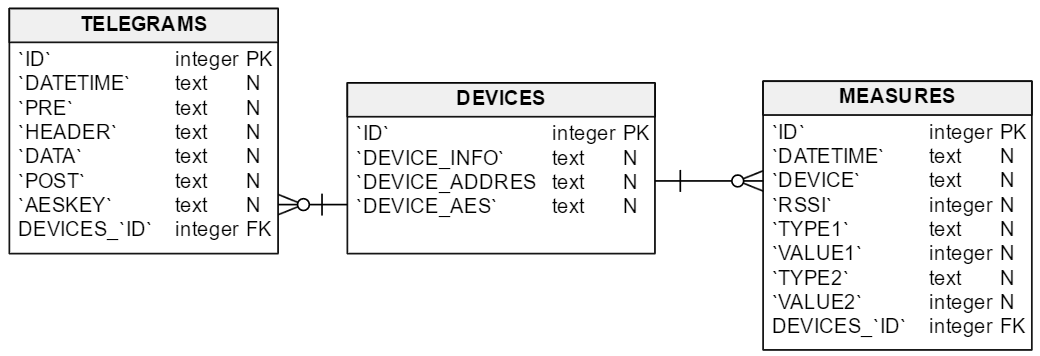
\includegraphics[scale=0.55]{obrazky/aplikace_databaze}
  \end{center}
	\vspace{-10pt}
  \caption{Model zvolené SqLite databáze}
	\label{databazovy_model}
	\vspace{-30pt}
\end{figure}
	
\section{Zajištění vizualizace dat}	
Zachycená a uložená data lze vykreslovat do grafů. Zvoleno bylo Google Charts API~\cite{uvod_google_charts_api} běžící na webovém serveru Apache2 a generovaném pomocí PHP/Pythonu. Pro tyto potřeby je nutné doinstalovat následující balíčky:
 
\begin{lstlisting}[style=MyCodeBash]
		sudo apt-get update
		sudo apt-get install apache2
		sudo apt-get install php7.0 
	\end{lstlisting}

Dále je nezbytné do umístění \texttt{$\backslash$var$\backslash$www$\backslash$html$\backslash$} nahrát zdrojové soubory visualizační aplikace. 

\section{Struktura aplikace}
Vzhledem k výše uvedeným požadavakům a technologiím byla zvolena struktura aplikace znázorněná na schématu přílohy~\ref{AplikaceDiagram}. Diagram je pro přehlednost odlišen barevnými bloky:
\begin{itemize}
	\item modrou barvou je znázorněna kostra programu,
	\item zelenou barvou je nekonečná smyčka naslouchání dat,
	\item růžovou barvou je případné dešifrování přenášených dat,
	\item červenou barvou jsou chyby znemožnující běh programu,
	\item oranžovou barvou jsou chyby znemožňující platnou analýzu či dešifrování daného telegramu a
	\item černou barvu je řízení samotného programu.
\end{itemize}

V následujících podkapitolách budou jednotlivé bloky aplikace představeny podrobněji.

\subsection{Start programu v rámci operačního systému}
Program je nyní spouštěn automaticky po startu operačního systému interpretem jazyka Python v příkazu screen. Tím je zajištěna nezávilost nasazení RaspberryPi a případných restartech zařízení. Ukončení programu nastává pouze násilným ukončením aplikace, restartem zařízení nebo závažnou chybou při startu programu. 

\subsection{Start programu z pohledu aplikace}
Program při startu kontroluje, zdali  má k dispozici všechny potřebné komponenty pro svůj běh. Program je závislý na knihovně PyCrypto, Serial nebo SQLite databázi.
Dále program kontroluje přítomnost a možnost otevření sériového portu. V případě úspěšného otevření portu je na něj zaslán příznak pro probuzení komunikačního modulu z úsporného režimu. Po probuzení následujě příkaz, který nastaví modul do režimu skeneru v komunikačním módu T1. Pokud některá z operací selže, je zaznamenán chybový stav a dojde k ukončení programu.

\subsection{Základní kontrola a cyklus příjmu dat}
Následně dojde ke spuštění smyčky naslouchání příchozích telegramů. Každý příchozí telgram je podroben sérii kontrol, pro ověření správnosti příjmu. Jako první je telegram podroben kontrole délky odpovídající sudým násobkům. Následně je telegram podroben základní analýze položek aplikační a linkové vrstvy. Dochází ke kontrole délky telegramu a jeho CRC součtu. Je provedena kontrola obsahu CI-pole, \texttt{Status} pole a \texttt{ConfigurationWord} pole. Pokud některá z položek neodpovídá, telegram je zaevidován a aplikace se vrátí do stavu čekání na příchod dalšího telegramu.
Na základě obsahu položky \texttt{ConfigurationWord} (viz Kap.~\ref{KapitolaConfigurationWord}) se program nadále větví na zpracování šifrovaného (Kap. \ref{KapitolaDesifrovani}) a nešifrovaného (Kap. \ref{KapitolaParsovani}) telegramu.

\subsection{Dešifrování dat}
\label{KapitolaDesifrovani}
%%%%%%%%%%%%%%%%%%%%%%%%%%%%%%%%%%%%%%%%%%%%%%%%%%%%%%%%%%
Pokud je analýzou položky \texttt{ConfigurationWord} zjištěno šifrování dat přenášených dat algoritmem AES128 CBC, je zahájen proces dešifrování dat.

Díky vnitřní implementaci IQRF modulu jsou všechny zachycené šifrované pakety automaticky rozšifrovány pomocí AES klíče nahraného v paměti modulu. Jedná se však o klíč daného modulu, nikoliv vyčítaného zařízení. Tato dešifrovaná data jsou tedy nevalidní. Celý postup dešifrování se tak komplikuje:

\begin{enumerate}
	\item Dojde ke stažení aktuálního AES klíče (viz Kap.~\ref{KapitolaStazeniKlice}) nastaveného v IQRF modulu, s pomocí něj a sestaveného inicializačního vektoru (viz Kap.~\ref{KapitolaInicializacniVektor})
jsou přijatá data zašifrována zpět do šifrovaného stavu jaký mají při přenosu, tedy data vyslaná daným měřícím zařízením, zašifrovaná AES klíčem daného měřícího zařízení.
	\item Pokud existuje, tak je z databáze načten odpovídající klíč příslušného měřícího zařízení a s pomocí již sestaveného inicializačního vektoru jsou data rozšifrována.
	\item Správnost rozšifrování se ověřuje pomocí kontrolních bajtů, v případě AES šifrování mají první dva bajty rozšifrovaných dat hodnotu 2Fh.
\end{enumerate}

Poté program s telegramem zachází jako s nešifrovaným, popsaným v Kap.~\ref{KapitolaParsovani}. Pokud není nalezen AES klíč odpovídajícího zařízení, pole \texttt{ConfigurationWord} obsahuje neimplementovaný algoritmus dešifrování či se proces dešifrování nezdaří, program vyvolá vyjímku, telegram je zaevidován a pokračuje se zpracováváním dalšího telegramu.

\subsection{Parsování dat}
\label{KapitolaParsovani}
Každý telegram je před svým zpracováním uložen do databáze, aby v případě potřeby (špatné dešifrování, neadekvátní dešifrovací klíč, chyba aplikace, neznámý senzor, \ldots) mohlo být provedeno nové zpracování daného telegramu. Poté je analyzováno M-Pole a v případě že se jedná o výrobce, jehož parsovací schéma je v této aplikaci implementováno, dochází k vyparsování přenášených hodnot. Následně v souladu s parsovacím schématem dochází k formátování a odpovídající interpretaci získaných dat (viz Kap.~\ref{PacketTableAnalysis}). Poté jsou získaná data uložena do databáze a zobrazena uživateli na výstup konzole.
Pokud parsování dat selže, dojde k výjimce, daný telegram je zaevidovánm v jeho zpracování se již nepokrečuje a aplikace se vrátí do stavu čekání na příchod dalšího telegramu.

\subsection{Uložení dat}
Správně interpretované hodnoty doplněné o časovou značku a informaci o měřícím zařízení jsou zapsány do databáze. Do této databáze se ukládají všechny příchozí validně zpracované telegramy, určené k pozdějšímu zpracování. Obohacení o časovou značku a údaje o zařízení je možné později tyto data efektivně třídit či v nich vyhledávat.

\subsection{Vizualizace dat}
Nad těmito daty se potom provádí vizualizace pomocí Google~Charts~API~\cite{uvod_google_charts_api}. To umožňuje interaktivní vykreslení a vyčítání uložných hodnot zachycených daným senzorem za vybraný časový úsek. Ukázky vizualizací zachycených dat jednotlivých zařízení jsou uvedeny v Příloze~\ref{PrilohaGrafy}.

\subsection{Ošetření výjimek}
Aplikace má ošetřeny dva chybové stavy. Hrubé chyby vedoucí k násilnému ukončení programu a lehké chyby znemožňující analýzu konkrétního telegramu. Hrubé chyby mohou vyvolat chybějící komponenty (databáze, komunikační modul, sériový port, \ldots), zatímco lehké chyby nastanou v případě, že daný telegram nemůže být zpracován (nevalidní příjem telegramu, neznámá struktura telegramu, neznámé zařízení, neznámý výrobce zařízení, neplatný šifrovací klíč, neplatné parsovací schéma, \ldots ), program vyvolá danou výjimku, zanechá zpracovávání aktuálního telegramu a následně přejde do stavu čekání na příchod dalšího telegramu.
Všechny tyto chyby jsou ukládány do příslušné tabulky v databázi, do chybového logu a taktéž sdělovány uživateli do konzole.

\subsection{Export dat}
V případě potřeby je vizualizační aplikace schopna dávkově vyexportovat uložená data určitého senzoru za daný časový úsek do Google Spreadsheets. Vzhledem k časové náročnosti při daném počtu naměřených hodnot je tato funkcionalita implementována spíše jako experimentální a v praxi se projevila jako nedostačující.


